\documentclass{standalone}

\usepackage{tikz}
    \usetikzlibrary{arrows.meta}

\usepackage{euscript} % Шрифт Евклида \EuScript{}
    \newcommand{\eS}{{\EuScript S}}
    
\begin{document}
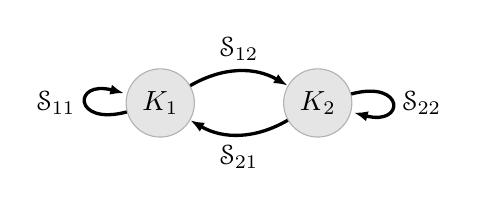
\begin{tikzpicture}
        \node[circle, draw=black!30, fill=black!10, shift={(0,0)}] (k1) {$K_1$};
        \node[circle, draw=black!30, fill=black!10, shift={(2,0)}] (k2) {$K_2$};
        \path[->,>={Latex[length=5pt]}, very thick]
            (k1) edge[bend left] node[above] {$\eS_{12}$} (k2)
            (k2) edge[bend left] node[below] {$\eS_{21}$} (k1)
            (k1) edge[loop left] node[left] {$\eS_{11}$} (k1)
            (k2) edge[loop right] node[right] {$\eS_{22}$} (k2);
    \end{tikzpicture}
\end{document}